\section{Performance Analysis of Parallelization Configurations}
\label{sec:parallelization_dimensions}

In this section, we consider the performance implications of combining pipeline and tensor model parallelism with data parallelism. Given a fixed budget of GPUs and batch size, one can use different degrees of the parallelism types in PTD-P to train models; each dimension exposes tradeoffs between memory footprint, device utilization, and amount of communication.

We discuss these tradeoffs in the rest of this section, and then show empirical results in \S\ref{sec:evaluation_parallel_configurations}. We present analytical models where relevant for the pipeline bubble size. We qualitatively describe how communication time behaves and present cost models for amount of communication; however, we do not present direct cost models for communication time, which is harder to model for a hierarchical network topology where interconnects between GPUs on the same server have higher bandwidth than interconnects between servers. To the best of our knowledge, this is the first work to analyze the performance \emph{interactions} of these parallelization dimensions.

\subsection{Notation}
We use the following notation in this section:
\begin{itemize}
    \item $(p, t, d)$: Parallelization dimensions. $p$ for the pipeline-model-parallel size, $t$ for the tensor-model-parallel size, and $d$ for the data-parallel size.
    \item $n$: Number of GPUs. We require $p \cdot t \cdot d = n$.
    \item $B$: Global batch size (provided as input).
    \item $b$: Microbatch size.
    \item $m=\frac{1}{b}\cdot\frac{B}{d}$: Number of microbatches in a batch \emph{per pipeline}.
\end{itemize}

\subsection{Tensor and Pipeline Model Parallelism}
Tensor and pipeline model parallelism can both be used to partition a model's parameters over multiple GPUs. As stated earlier, using pipeline parallelism with periodic flushes results in a pipeline bubble of size $(p-1) / m$. Let us assume that $d=1$ (data-parallel size); consequently, $t \cdot p = n$. The pipeline bubble size in terms of $t$ is:
$$\frac{p-1}{m} = \frac{n/t-1}{m}.$$
As $t$ increases, the pipeline bubble thus decreases for fixed $B$, $b$, and $d$ ($m = B / (b \cdot d)$ is fixed as well).

The amount of communication performed between different GPUs is also affected by the values of $p$ and $t$. Pipeline model parallelism features cheaper point-to-point communication. Tensor model parallelism, on the other hand, uses all-reduce communication (two all-reduce operations each in the forward and backward pass, see \S\ref{sec:tensor_model_parallelism}). With pipeline parallelism, the total amount of communication that needs to be performed between every pair of consecutive devices (for either the forward or backward pass) for each microbatch is $bsh$, where $s$ is the sequence length and $h$ is the hidden size. With tensor model parallelism, tensors of total size $bsh$ need to be all-reduced among $t$ model replicas twice each in the forward and backward pass for each layer, leading to a total communication of $8bsh \left(\frac{t-1}{t}\right)$ \emph{per layer} per device for each microbatch. Each device typically has multiple layers; the total amount of tensor-parallel-communication per device for each microbatch is then $l^{\text{stage}} \cdot \left(8bsh \left(\frac{t-1}{t}\right)\right)$, where $l^{\text{stage}}$ is the number of layers in a pipeline stage.

Consequently, we see that tensor model parallelism increases the amount of communication between devices. Thus, when $t$ is larger than the number of GPUs in a single node, the overhead of performing tensor model parallelism across slower inter-node links can be impractical. We see these results empirically in \S\ref{sec:evaluation_parallel_configurations}.

\vspace{0.1in}
\noindent\fbox{\parbox{0.98\columnwidth}{\textbf{Takeaway \#1:} When considering different forms of model parallelism, tensor model parallelism should generally be used up to degree $g$ when using $g$-GPU servers, and then pipeline model parallelism can be used to scale up to larger models across servers.}}

\subsection{Data and Model Parallelism}
\label{sec:data_and_model_parallelism_analytical_model}

We also want to consider the interaction between data parallelism and the two types of model parallelism. In this section, we consider these interactions independently for simplicity.

\begin{figure}[t!]
    \centering
    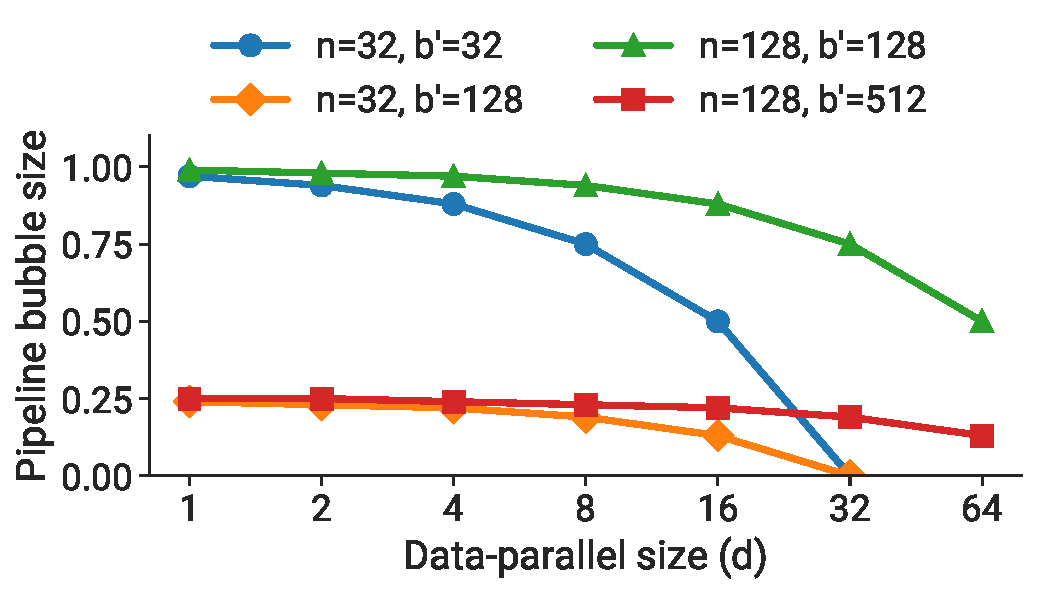
\includegraphics[keepaspectratio=1.0,width=0.9\columnwidth]{figures/pipeline_bubble_size_data_and_pipeline_parallelism.pdf}
    \vspace{-0.1in}
    \caption{
         Fraction of time spent idling due to pipeline flush (pipeline bubble size) versus data-parallel size ($d$), for different numbers of GPUs ($n$) and ratio of batch size to microbatch size ($b' = B/b$).
    }
    \vspace{-0.1in}
    \label{fig:pipeline_bubble_size_data_and_pipeline_parallelism}
\end{figure}

\subsubsection{Pipeline Model Parallelism} Let $t=1$ (tensor-model-parallel size). The number of microbatches per pipeline is $m = B / (d \cdot b)=b'/d$, where $b':=B/b$. With total number of GPUs $n$, the number of pipeline stages is $p=n/(t\cdot d)=n/d$. The pipeline bubble size is:$$\frac{p-1}{m} = \dfrac{n/d-1}{b'/d} = \dfrac{n-d}{b'}.$$
As $d$ becomes larger, $n-d$ becomes smaller, and thus the pipeline bubble becomes smaller. Figure~\ref{fig:pipeline_bubble_size_data_and_pipeline_parallelism} shows the behavior of the pipeline bubble size for various values of $d, n,$ and $b'$. It might not be possible to increase $d$ all the way to $n$ for all models, since a model's full training memory footprint might be larger than the memory capacity of a single accelerator.

Overall throughput will thus increase if the all-reduce communication needed for data parallelism does not drastically increase with higher $d$, which should hold since the communication time for a ring-based implementation scales with $\frac{d-1}{d} = 1 - \frac{1}{d}$.

We can also analyze the impact of increasing the batch size $B$. For a given parallel configuration, as the batch size $B$ increases, $b'=B/b$ increases, $(n-d)/b'$ decreases, consequently increasing throughput. All-reduce communication required by data parallelism also becomes more infrequent, further increasing throughput.

\subsubsection{Data and Tensor Model Parallelism}
With tensor model parallelism, all-reduce communication needs to be performed for \emph{every} microbatch. This can be expensive across multi-GPU servers. On the other hand, data parallelism only needs to perform expensive all-reduce communication \emph{once per batch}. Moreover, with tensor model parallelism, each model-parallel rank performs a subset of the computation in each model layer, and thus for insufficiently-large layers, modern GPUs might not perform these sub-matrix computations with peak efficiency.

\vspace{0.1in}

\noindent\fbox{\parbox{0.98\columnwidth}{\textbf{Takeaway \#2:} When using data and model parallelism, a total model-parallel size of $M = t \cdot p$ should be used so that the model's parameters and intermediate metadata fit in GPU memory; data parallelism can be used to scale up training to more GPUs.}}

\subsection{Microbatch Size}
\label{sec:microbatch_size_analytical_model}

\begin{figure}[t!]
    \centering
    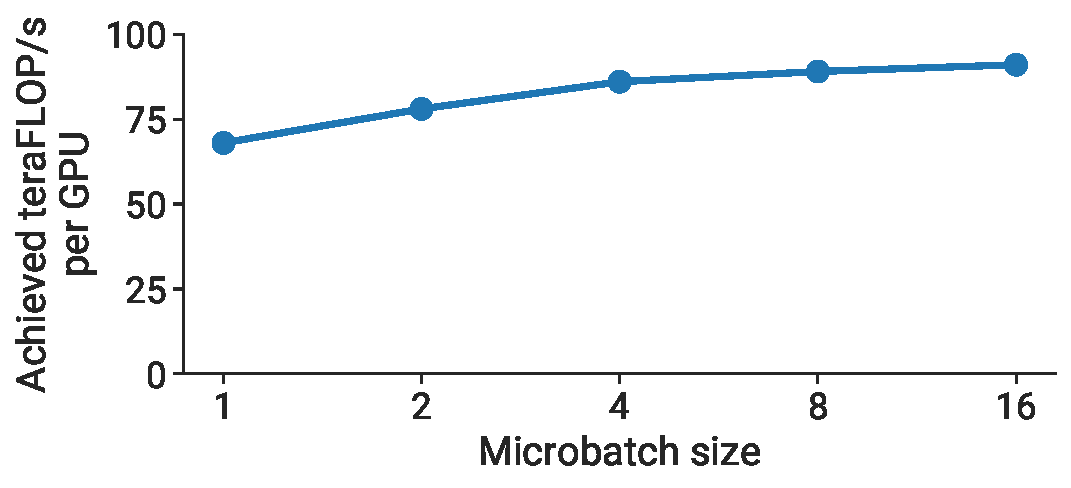
\includegraphics[keepaspectratio=1.0,width=0.9\columnwidth]{figures/throughput_vs_microbatch_size.pdf}
    \vspace{-0.1in}
    \caption{
         Per-GPU throughput versus microbatch size for a GPT model with a billion parameters (128 attention heads, hidden size of 4096, 4 transformer layers).
    }
    \vspace{-0.1in}
    \label{fig:throughput_vs_microbatch_size}
\end{figure}

\begin{figure}[t!]
    \centering
    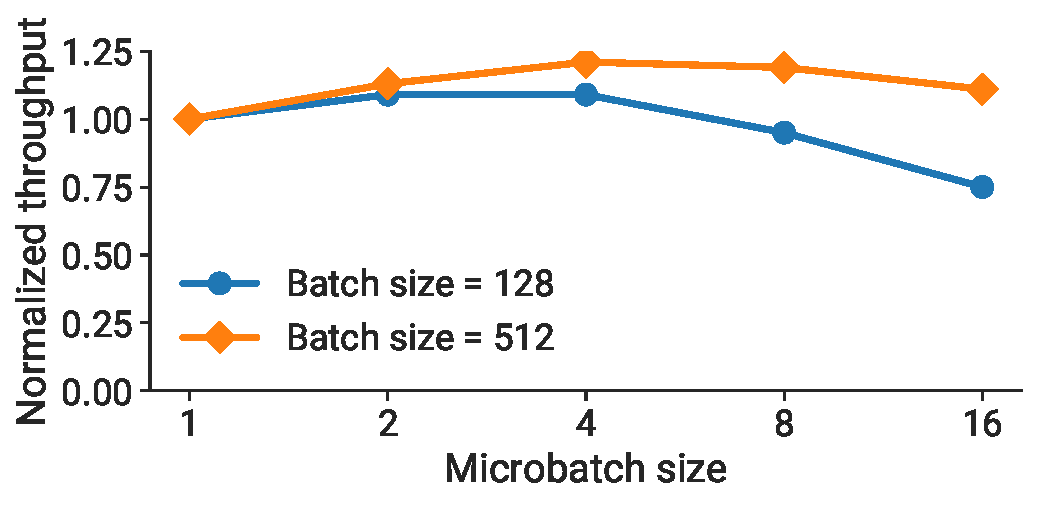
\includegraphics[keepaspectratio=1.0,width=0.9\columnwidth]{figures/per_batch_time_estimate_vs_microbatch_size.pdf}
    \vspace{-0.1in}
    \caption{
         Behavior of normalized estimated throughput  (time computed as $t = \left(b' / b + p - 1\right) \cdot \left(t_f(b) + t_b(b)\right)$) with respect to the microbatch size $b$ for the same GPT model from Figure~\ref{fig:throughput_vs_microbatch_size}.
    }
    \vspace{-0.1in}
    \label{fig:per_batch_time_estimate_vs_microbatch_size}
\end{figure}

The choice of the microbatch size $b$ also affects model-training throughput. For example, we see in Figure~\ref{fig:throughput_vs_microbatch_size} that per-GPU throughput increases by up to $1.3\times$ with a larger microbatch size on a single GPU. We now want to determine the optimal microbatch size $b$ given a parallel configuration $(p, t, d)$ and batch size $B$. The amount of data-parallel communication will be the same regardless of the microbatch size. Given functions $t_f(b)$ and $t_b(b)$ that map the microbatch size to the forward and backward computation times for a single microbatch, the total time spent computing a batch, ignoring communication cost, is (as before, define $b'$ as $B/d$):
\begin{equation}
    \left(b' / b + p - 1\right) \cdot \left(t_f(b) + t_b(b)\right). \label{equation:processing_time_estimate}
\end{equation}
The microbatch size thus affects both the arithmetic intensity of operations as well as the pipeline bubble size (by affecting $m$). Figure~\ref{fig:per_batch_time_estimate_vs_microbatch_size} shows estimated throughput (equation (\ref{equation:processing_time_estimate}) used to estimate processing time) for a GPT model with a billion parameters and $(p, t) = (8, 8)$. The optimal $b$ for both batch sizes is 4.

\vspace{0.1in}
\noindent\fbox{\parbox{0.98\columnwidth}{\textbf{Takeaway \#3:} The optimal microbatch size $b$ depends on the throughput and memory footprint characteristics of the model, as well as the pipeline depth $p$, data-parallel size $d$, and batch size $B$.}}

\subsection{Activation Recomputation}

Activation recomputation~\cite{huang2019gpipe, chen2016training, griewank2000algorithm, mlsys2020_196} is an optional technique that trades off an increase in the number of compute operations performed for additional memory footprint, by running the forward pass a second time just before the backward pass (and stashing only the input activations for a given pipeline stage, as opposed to the entire set of intermediate activations, which is much larger). Activation recomputation is required to train reasonably large models with pipeline parallelism to keep memory footprint acceptably low. Previous work like PipeDream-2BW~\cite{narayanan2021memory} has looked at the performance ramifications of activation recomputation. 

The number of activation checkpoints does not impact throughput, but impacts memory footprint. Let $A^\text{input}$ be the size of the input activations of a layer, and $A^\text{intermediate}$ be the size of intermediate activations per layer. If a model stage has $l$ layers, and if $c$ is the number of checkpoints, the total memory footprint is going to be $c \cdot A^\text{input} + l/c \cdot A^\text{intermediate}$. The minimum value of this function is obtained when $c = \sqrt{l \cdot \left(A^\text{intermediate} / A^\text{input}\right)}$. In practice, we measure $A^\text{intermediate}$ empirically. For most cases, checkpointing every 1 or 2 transformer layers is optimal.

Other techniques such as activation partitioning~\cite{rajbhandari2019zero} can also be used in conjunction with tensor model parallelsim to reduce the memory footprint due to activations further.